\begin{figure}
\centering
\begin{subfigure}[b]{0.5\textwidth}
    \centering
    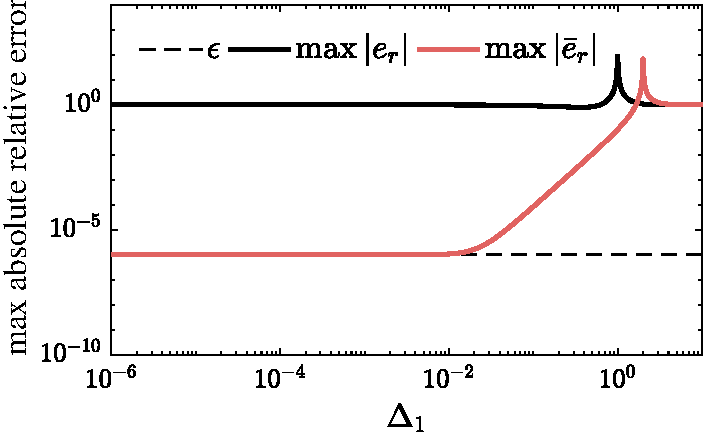
\includegraphics[width=\textwidth]{../ch4/figures/dt_errors_1}
    \caption{$y_0 = 10^{-6}$ and $a = 2$.\label{fig:ch4:dt_errors_1}}
\end{subfigure}%
\begin{subfigure}[b]{0.5\textwidth}
    \centering
    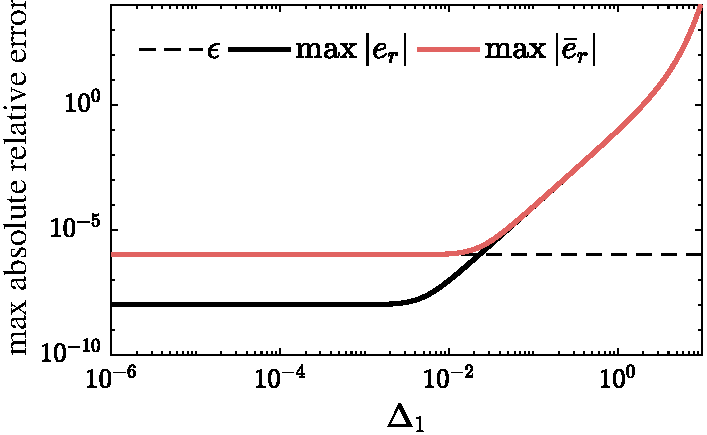
\includegraphics[width=\textwidth]{../ch4/figures/dt_errors_2}
    \caption{$y_0=10^2$ and $a=-1$.\label{fig:ch4:dt_errors_2}}
\end{subfigure}
\caption[Maximum absolute relative error vs. step size for defect constraints]{Maximum absolute relative error vs. step size for original and scaled defect constraints.\label{fig:ch4:dt_errors}}
\end{figure}
